%% LaTeX file for Design representation

%% design.tex
%% 
%% Karlsruhe Institute of Technology
%% Version 1.0, 2018-12-13

%% Available page modes: oneside, twoside
%% Available languages: english, ngerman
%% Available modes: draft, final (see README)
\documentclass[oneside, english, final]{design}

\usepackage{graphicx}
\usepackage{caption}
\usepackage{pdfpages}
\usepackage[export]{adjustbox}
\usepackage{hyperref}

\hypersetup{hidelinks,
backref=true,
pagebackref=true,
hyperindex=true,
breaklinks=true,
colorlinks=true, linkcolor=black,
urlcolor=blue,
bookmarks=true,
bookmarksopen=false,
pdftitle={Title},
pdfauthor={Author}}

%usepackage{lipsum}


%% ---------------------------------
%% | Information about the thesis  |
%% ---------------------------------

%% Name of the author
\author{PSE Group}

%% Title (and possibly subtitle) of the thesis
\title{Real-time visualization of analyzed industrial communication network traffic\\ \hfill \\Implementation Report}

%% Type of the thesis 
%\thesistype{PSE}

%% The advisors are PhD Students or Postdocs
\advisor{M.Sc. Ankush Meshram}
%\begin{document}


%\end{document}
\thispagestyle{empty}

\settitle

%% --------------------------------
%% | Settings for word separation |
%% --------------------------------

%% Describe separation hints here.
%% For more details, see 
%% http://en.wikibooks.org/wiki/LaTeX/Text_Formatting#Hyphenation
\hyphenation{
% me-ta-mo-del
}

%% --------------------------------
%% | Bibliography                 |
%% --------------------------------

%% Use biber instead of BibTeX, see README
\usepackage[citestyle=numeric,style=numeric,backend=biber]{biblatex}
\usepackage{microtype}

\addtolength{\belowcaptionskip}{-10pt}
\setlength{\textfloatsep}{10pt plus 1.0pt minus 2.0pt}
%\addtolength{\abovecaptionskip}{-100pt}
\frenchspacing
%% ====================================
%% ====================================
%% ||                                ||
%% || Beginning of the main document ||
%% ||                                ||
%% ====================================
%% ====================================
\begin{document}
\nocite{*}

%% Set PDF metadata
\setpdf

%% Set the title
\maketitle

%% ----------------
%% |   Abstract   |
%% ----------------

\hfill

\begin{center}
	\large{Version 1.0.0}
\end{center}


%% The text is included from the following files:
%% - sections/abstract
\thispagestyle{empty}
\begin{abstract}
	\thispagestyle{empty}
\end{abstract}

%% -----------------
%% |   Main part   |
%% -----------------
\thispagestyle{empty}
\newpage
\thispagestyle{empty}
\tableofcontents
\cleardoublepage
\setcounter{page}{1}


\section{Design}\label{sec:intro}
\subsection{Introduction}

This implementation report covers changes in the design from the one decribed in the original design phase
and decribes the current state of the implementation by lists of completed and not completed requirements.


\subsection{Changes in the Design}

Changes are grouped together according to the reason for the change.

\subsubsection{User Interface changes for better aesthetics and convenience}
\begin{itemize}
  \item{New Login Page
  \\
    Opted for a different graphical design than the one in the mockups due to aesthetic reasons. The functionality and behavior of the login page remains the same as in the design docs.}
    
  \item{Removal of the filter button inside diagram control containers
  \\
  The filters now can be easily accessible inside the config modal of the diagram.}
\end{itemize}

\subsubsection{User Interface changes for usability improvements}
\begin{itemize}
  \item{New text input box for WebSocket endpoint
  \\
  Added the feature of choosing an arbitrary WebSocket endpoint by persisting the input with Browser Local Storage API, making the frontend application completely standalone and therefore largely simplified the deploy process of the entire DHSTTOS suite.}
  
\end{itemize}

\subsubsection{Refactoring for cleaner code and changes for convenience reasons}
\begin{itemize}
\item{Data formatting helper function on the frontend
  \\
  Added a helper function \textsf{\textbf{formatData = (\{ groupName, x, y, rawData = [] \}) : Object[] }} which converts the raw data points the frontend receives from the server to structured data arrays which allows easy data passing into the diagram drawing routines.}
  
\item{Add parameter
  \\
	Added parameter DBname to \textsf{\textbf{MongoConsumer(user, pass, dbName)}} for creating a reference to pass onto the MongoClientMediator}

\item{Refactoring
  \\
  Add attribute \textsf{\textbf{private KafkaConsumer<String, String> consumer}} because other functions need to use the consumer}

  \item{Refactor: extract instance attribute}
    \\ 
    Add attribute \textsf{\textbf{private MongoDatabase db}}
    as a reference to the database all methods need to access.

  \item{Convenience functions for different data types}
    \\
    Added variations of \textsf{\textbf{addRecordToCollection(Record record, String collection)}}
    that take a document or an list of documents or an array of record sinstead of a Record.


  \item{Add convenience function}
    \\
    Added \textsf{\textbf{getCollectionAsRecordsArrayList()}}
    to DataProcessor.

  \item{Refactor passing the current mediator object}
  \\
    Add parameter \textsf{\textbf{MongoClientMediator}} to \textsf{\textbf{public static void ProcessData:processData(String collectionName, MongoClientMediator clientMediator)}} so that \textsf{\textbf{processData}} can use it to write the processed data to the database. Remove attribute \textsf{\textbf{ProcessData:MongoClientMediator client}} which was used for this before.


  \item{Add convenience function}
    \\
    Add method \textsf{\textbf{public static void processData(ArrayList<String> collectionNames, MongoClientMediator clientMediator)}} to process a list of collections (instead of calling \textsf{\textbf{processData}} for each collection.
    
  \item{Add convenience function}
    \\
    Added method \textsf{\textbf{public Document getNewAggregatorDocument(Date tstmp)}} for easier handling of date values.

    
  \item{Add convenience attributes}
    \\
    Add the variables Variables
    \textsf{\textbf{private ArrayList<Map<String, Object>> connectionsMapList}} and
    \textsf{\textbf{private Document currentDocument}} to the classes \textsf{\textbf{FlowRatePerSecond}} and \textsf{\textbf{NumberOfConnectionsPerNode}} to
    keep track of which document is being processed now and which connections happened within this second.


\item{Refactoring for cleaner code in protocol handling}
  \\
  Change the protocol parsing in class \textsf{\textbf{ClientProtocoHandler}} from a switch construct to using a private enum.

\end{itemize}

\subsubsection{Changes due to clarified requirements}
\begin{itemize}
\item{Differing input formats for Date/Timestamp}
  \\
  Split class \textsf{\textbf{PacketRecord}} into \textsf{\textbf{PacketRecordDesFromMongo}} and \textsf{\textbf{PacketRecordDesFromKafka}} to handle different formats.

\end{itemize}


\subsubsection{Changes due to oversights}

These are changes and additions due to oversights and mistakes in the original design.

\begin{itemize}
  \item{added dbName to MongoClientMediator since we need to know from which DB we want to read/write collections.}
\\

  \item{Unspecified return type}
    \\
    The return type of \textsf{\textbf{public ArrayList<Document> processData( ArrayList<Record> records)}} in \textsf{\textbf{IAggregator}}
was unspecified in the Design document.

  \item{Session handling}
    \\
    To handle session state, \textsf{\textbf{Hub:login()}}, \textsf{\textbf{Hub:loginWithToken()}}, and \textsf{\textbf{Hub:logout()}} were added.
    To keep track of client session state, the private attributes \textsf{\textbf{Hub:sessions}} and \textsf{\textbf{Hub:loginTokens}} were added.

\end{itemize}


\subsubsection{Changes due to unexpected complexity}
These changes can be attributed to lack of familiarity with the used components and libraries.
\begin{itemize}
  \item{Workaround for Kafka's API}
    \\
    Change \textsf{\textbf{getAllTopics()}} to \textsf{\textbf{getAllTopicsPartitions()}}:
    return a Collection of topic partitions essentially to force kafka to send all records from the start.
    It was complex to make kafka read all the topics from the beginning.
    Secondary aspect: convenient because it relegates topic creation to another method.

  \item{Workaround for Kafka's API}
    \\
    Add method \textsf{\textbf{ArrayList<String> getTopicsForProcessing()}}
  because there are some topics in kakfka which are for internal use, e.g. \_\_consumeroffsets.
 This returns the topics we need to process.
	
  \item{Exception handling}
    \\ 
    The constructor for class \textsf{\textbf{MongoClientMediator}} now throws a LoginFailureException instead of forwarding an unchecked exception.

  \item{Converting between different APIs}
    \\ 
    Add method \textsf{\textbf{mongoIteratorToStringArray(MongoIterable)}}
    because the hub expects an array but the mongodb returns a MongoIterable.

  \item{Making the network protocol more expressive to simplify handling responses}
  \item{Handling the login happening in another websocket session than the main app}
    \\
    \begin{itemize}
    To deal with a restart of the websocket connection when changing from the login page to the main page, session handling was changed. Added the \textsf{\textbf{LOGIN\_TOKEN}} request to the protocol and \textsf{\textbf{Hub:loginWithToken}}.
  Also, the client can add new key-value-pairs to the request which will be returned unchanged by the server.

    \end{itemize}

  \item{Adapt to React and MobX}
    \\
    To adapt to the observer-driven architecture of React and MobX, store data from the server in datastructures \textsf{\textbf{dataStore.rawData}} and \textsf{\textbf{dataStore.alarms}}
    instead of returning it as return values of
    \textsf{\textbf{getAvailableCollections()}},
    \textsf{\textbf{getCollection()}}, \textsf{\textbf{getCollectionSize()}}, \textsf{\textbf{getRecordsInRange()}} and \textsf{\textbf{getRecordsInRangeSize()}} in \textsf{\textbf{wsutils.js}}.

\end{itemize}

\newpage

\subsection{List of implemented must- and should-requirements}
\subsubsection{List of implemented must-requirements}
FR100, FR110, FR200, FR300, FR400, FR500, FR700, FR710, FR720, FR1110, FR1300, FR1310
\\
cancelled after Mike left: FR800

\subsubsection{List of implemented should-requirements}
\begin{itemize}
  \item{FR1332 filter to compute flow rate}
  \begin{itemize}
    \item{this has instead been implemented in the backend which provides this as a new data stream}
  \end{itemize}
  \item{FR1400}
\end{itemize}

\subsubsection{List of not implemented must-requirements}
\begin{itemize}
  \item{FR600 dynamically change the selected/displayed components}
  \item{FR900 The amount of data can be limited via a slider [...]}
to which all diagrams must update to.
  \item{FR910 Within the slider the user is able to scroll through the timeline and the diagrams need to react in real-time.}
  \item{FR1000 auto scroll}
  \item{FR1100 pick data points, hover}
  \item{FR1200 selecting data points}
  \item{FR1210 create new diagram from selected data}
  \item{FR1330}
\end{itemize}


\subsubsection{List of not implemented should-requirements}
\begin{itemize}
\item{FR1320 per-diagram filters}
\end{itemize}


\subsection{Timeline and Delays}
There were delays in the implementation phase caused by
\begin{itemize}
\item{clarification of requirements}
\item{evaluation of graphics libraries}
\item{familiarization with the used APIs and libraries}
\end{itemize}

\begin{figure}[h!]
	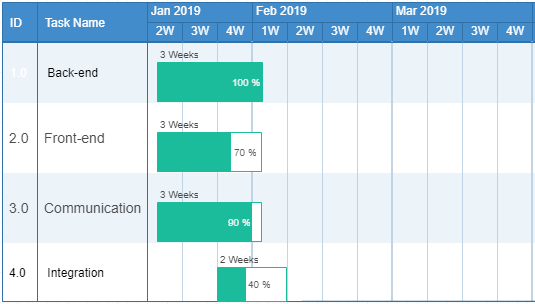
\includegraphics[max size={\textwidth}{\textheight}]{implementation-gantt1.png}
	\caption{The timeline.}
	\label{fig:gantt1}
\end{figure}


\subsection{Overview of unit tests}
Number of unit tests:\\
\hfill
\\
\begin{tabular}{|p{0.8\textwidth}p{0.1\textwidth}}
DataProcessor & 2\\  Test 1 and 2 both test the functionality of trying to process missing data. In both cases the aggregators responsible should not fail and simply make sure nothing gets added into the Database.\\ \\
Hub & 4\\ Test session handling methods.\\ \\
MockMongoDBUserSession & 4\\ \\
MongoClientMediator & 5 \\ Test1 and 2 and 3: test different credential errors, like missing credentials or credential without access to the necessary databases. All tests cases return a LoginFailureException.\\ 
Test 4 and 5 test handling null reference objects to adding records into MongoDB. In this case then simply, nothing is added into the database.\\ \\
MongoConsumer & 2 \\ Test 1 : tests the case on failure to communicate with kafka, the consumer exists and reports this to the console but operation of all other parts of the program continue since failure of this does not affect working with data already stored in the database.\\
Test2: tests case when the consumer does not have the right credentials to access the MongoDB, the Consumer should then fail to be created and call a LoginFailureException.\\ \\
TestClientProtocolHandler & 2 \\ \\
FormatData. & \\ Testing the GUI would be possible however, this is both complex and time consuming. Due to time constraints minimal testing was done outside of basic functionality.\\ \\
\end{tabular}


\end{document}
